\documentclass[a4paper,12pt]{scrartcl}

\usepackage[T1]{fontenc}
\usepackage{lmodern}
\usepackage[utf8]{inputenc}
\usepackage[french]{babel}
\usepackage{graphicx}
\usepackage{microtype} 
\usepackage[onehalfspacing]{setspace}
\usepackage[top=2.5cm, bottom=2.5cm, left=3cm, right=3.5cm]{geometry}
\usepackage{tabularx}
\usepackage{graphicx}
\usepackage{longtable}
\usepackage{listings}
\usepackage{listingsutf8}
\usepackage{dsfont}
\usepackage{appendix}
\usepackage{amsmath}
\usepackage{hyperref}
\usepackage{mathtools, amssymb}
\usepackage[usenames,dvipsnames]{color}

% \begin{equation}
% \begin{split}
%     \dbx & =\dbx[3cm] \\
%     & =\dbx
% \end{split}
% \end{equation}

\definecolor{MyDarkGreen}{rgb}{0.0,0.4,0.0}
\lstloadlanguages{Matlab}
\lstset{language=Matlab,                        % Use MATLAB
        frame=single,                           % Single frame around code
        basicstyle=\small\ttfamily,             % Use small true type font
        keywordstyle=[1]\color{Blue}\bfseries,  % MATLAB functions bold and blue
        keywordstyle=[2]\color{Purple},         % MATLAB function arguments purple
        keywordstyle=[3]\color{Blue}\underbar,  % User functions underlined and blue
        identifierstyle=,                       % Nothing special about identifiers
                                                % Comments small dark green courier
        commentstyle=\usefont{T1}{pcr}{m}{sl}\color{MyDarkGreen}\small,
        stringstyle=\color{Purple},             % Strings are purple
        showstringspaces=false,                 % Don't put marks in string spaces
        tabsize=5,                              % 5 spaces per tab
        %
        %%% Put standard MATLAB functions not included in the default
        %%% language here
        morekeywords={xlim,ylim,var,alpha,factorial,poissrnd,normpdf,normcdf},
        %
        %%% Put MATLAB function parameters here
        morekeywords=[2]{on, off, interp},
        %
        %%% Put user defined functions here
        morekeywords=[3]{brownmo},
        %
        morecomment=[l][\color{Blue}]{...},     % Line continuation (...) like blue comment
        numbers=left,                           % Line numbers on left
        firstnumber=1,                          % Line numbers start with line 1
        numberstyle=\tiny\color{Blue},          % Line numbers are blue
        stepnumber=5,                           % Line numbers go in steps of 5
        literate=%                              % accents and Umlaute
                 {Ö}{{\"O}}1
                 {Ä}{{\"A}}1
                 {Ü}{{\"U}}1
                 {ß}{{\ss}}1
                 {ü}{{\"u}}1
                 {ä}{{\"a}}1
                 {ö}{{\"o}}1
                 {\$}{{\dollar}}1
        }

\title{Mini projet 1: Calcul du prix d'une option asiatique}
\author{Valentin DE CRESPIN DE BILLY \\ Matthias LANG}
\date{30.11.2021}

\linespread{1.5} 


\begin{document}

\maketitle
\begin{center}

  \thispagestyle{empty}

  N. d'étudiant: 247067 et 313411\\
  Université Catholique de l'Ouest\\
  Mathématiques financières

\end{center}

\newpage

\section{Calculer le prix du sous-jacent}

Nous avons essayé d'atteindre une équation qui ne dèpend que des variables connues comme la formule de Black-Scholes.
Cela n'a pas fonctionné.

\begin{align}%equation} \label{1} 
dS_t  &=  S_t(rdt+\sigma \sqrt{S_t} dW_t) \\
     \iff \frac{dS_t}{S_t}  &=  rdt+\sigma \sqrt{S_t} dW_t
\end{align}


On prend l'équation 1:
%\begin{equation} \label{3}
%\begin{multlined}
\begin{align*}
= dS_t~=~S_trdt+\sigma S_t^{1.5} dW_t ~~
\text{; Puis} \\
d \langle S_t &, ~ S_t\rangle \\
=\langle dS_t &,~ dS_t\rangle ~=\\
=\langle S_trdt+\sigma S_t^{1.5} dW_t &,~
         S_trdt+\sigma S_t^{1.5} dW_t \rangle ~=\\
=\langle \sigma S_t^{1.5} dW_t &,~
         \sigma S_t^{1.5} dW_t \rangle ~=\\
=S_t^3 \sigma^2 \langle dW_t &,~  dW_t \rangle ~=\\
=S_t^3 \sigma^2 dt
\end{align*}


On pose: 
$X_t = ln(S_t)$
%\begin{equation} \label{4}
%\begin{multlined}
\begin{align}
\text{Formule d'Ito: } dln(S_t) = \frac{dS_t}{S_t} + \frac{1}{2} \frac{-1}{S_t^2}d \langle S_t, ~S_t \rangle \\
\end{align}
Avec les équations 2 et 3:
\begin{align}
dln(S_t) = 
rdt + \sigma \sqrt{S_t} dW_t - \frac{1}{2}S_t \sigma^2 dt =
(r - \frac{1}{2}S_t\sigma^2)dt + \sigma\sqrt{S_t}dW_t
\end{align}


\begin{align*}
ln( \frac{S_t}{S_0} ) 
&= ln(S_t)-ln(S_0) = \int_0^t dln(S_u) = \\
&= \int_0^t (r-\frac{1}{2} S_t \sigma^2)du~+~\int_0^t \sigma \sqrt{S_t}dW_t \\
&=\dots
\end{align*}
Donc on ne peut pas facilement dériver une formule pour le prix comme ça, qui dépend que des variables fixées, mais on peut le simuler pas à pas en utilisant (1):

\begin{equation} \label{6}
\begin{split}
S_0  &~\text{soit connu} \\
dS_0 &= S_0(rdt + \sigma \sqrt{S_0} dW_0) \\
S_1  &\approx S_0 + dS_0 \\
dS_1 &= S_1(rdt + \sigma \sqrt{S_1} dW_1) \\
S_2  &\approx S_1 + dS_1 \\
\dots
\end{split}
\end{equation}



\subsection{Réduction de la variance du éstimateur}

Les éstimateurs ont une variance telle que:
$ \hat{Var}(C) = \hat{\sigma_i^2} / n_t$, oú $n_t$ est le nombre des observations et $\hat{\sigma_i^2}$ est la variance estimée de la population, qui est égal à la variance de l'échantillon.

Supposons que nous ne connaissions ni les paramètres ni la règle à partir desquels les prix sont établis. 
Nous ne pouvons donc pas augmenter le nombre d'observations pour améliorer l'estimateur.
Quelle autre possibilité existe-t-il pour réduire sa variance ?

Avec les techniques de bootstrap on pourrait répliquer les données. 
Mais on risque de introduir un biais.
Si on utilise une variable de contrôle on n'invente pas des nouvelles données, ni risque-t-on de changer l'ésperance.

% variable antith

\section{Réalisation numerique}

Les algorithmes sont réalisées avec deux langues de programmation: Matlab et Visual Basic for Applications.
Plusieurs graphiques sont y générés, vous les trouverez dans l'annexe \ref{graphiques}.
En plus, avec le logiciel Excel nous avons crée un dashboard, voir une capture d'figure ref{X}. 
Vous trouverez les scriptes et les images dans l'annexe, et avec la fiche de dashboard également dans le \href{https://github.com/matthias-10/UCO_actuariat_mini-projet}{repository}.

%%%%%%%% A N N E X E %%%%%%%%%%%%%%%%%%
\clearpage

\appendix
\appendixpage
\addappheadtotoc

\begin{center}
Toutes les fiches se trouvent dans le repository en ligne: 

 \url{https://github.com/matthias-10/UCO_actuariat_mini-projet}
\end{center}

\section{Graphiques} \label{graphiques}

\begin{figure}[h!]
  \begin{center}
    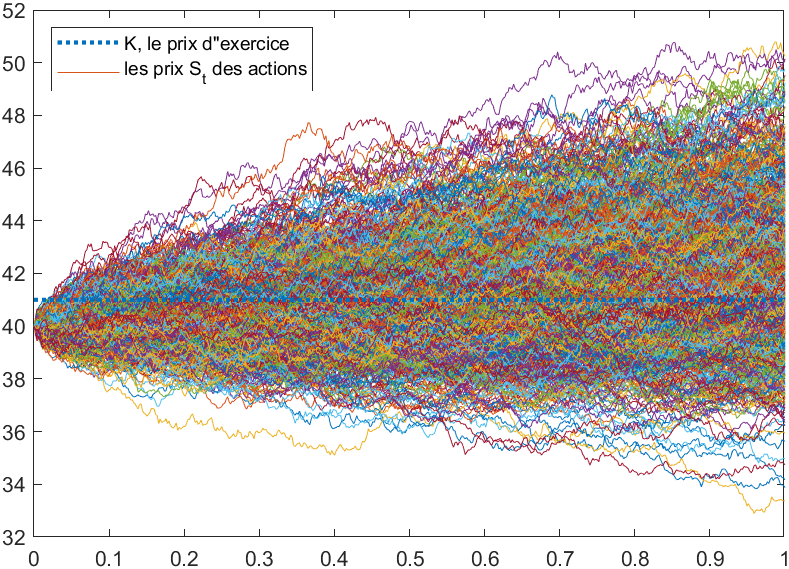
\includegraphics[width=14cm]{"graphiques/S.png"}
    \caption{Les graphes de tous trajectoires, plotés avec matlab}
    \label{fig:S}
  \end{center}
\end{figure}

\begin{figure}[h!]
  \begin{center}
    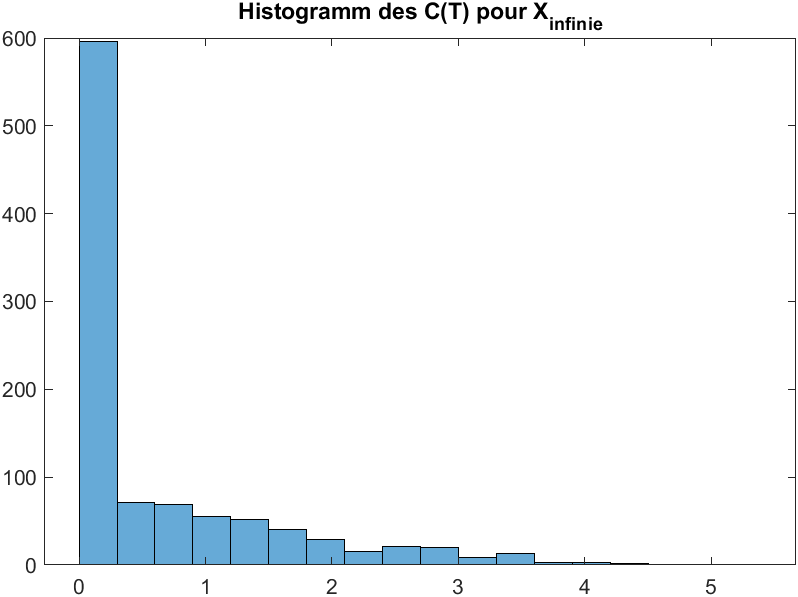
\includegraphics[width=14cm]{"graphiques/hist_C_inf.png"}
    \caption{Histogramme des simulations pour $C_{\infty}$}
    \label{fig:hist_C_inf}
  \end{center}
\end{figure}

\begin{figure}[h!]
  \begin{center}
    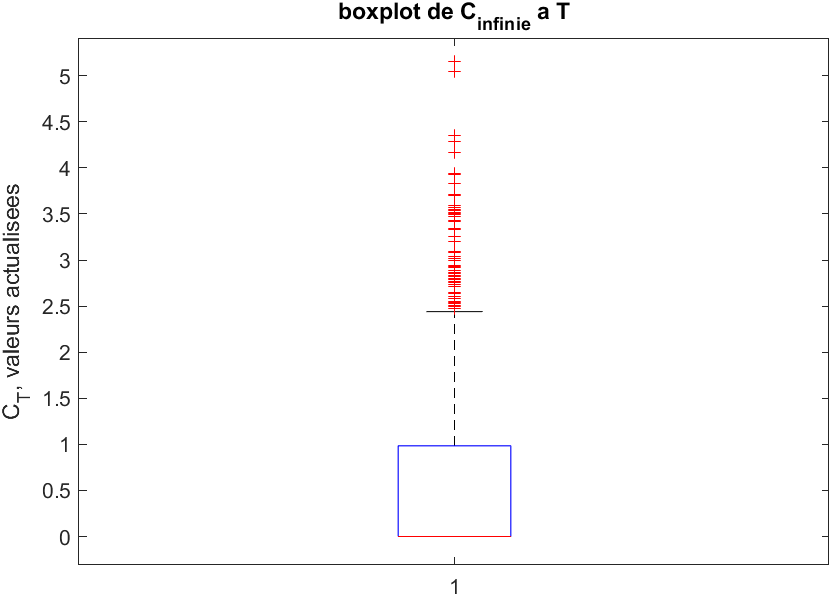
\includegraphics[width=14cm]{"graphiques/box_C_inf.png"}
    \caption{Boxplot des simulations pour $C_{\infty}$}
    \label{fig:box_C_inf}
  \end{center}
\end{figure}

\begin{figure}[h!]
  \begin{center}
    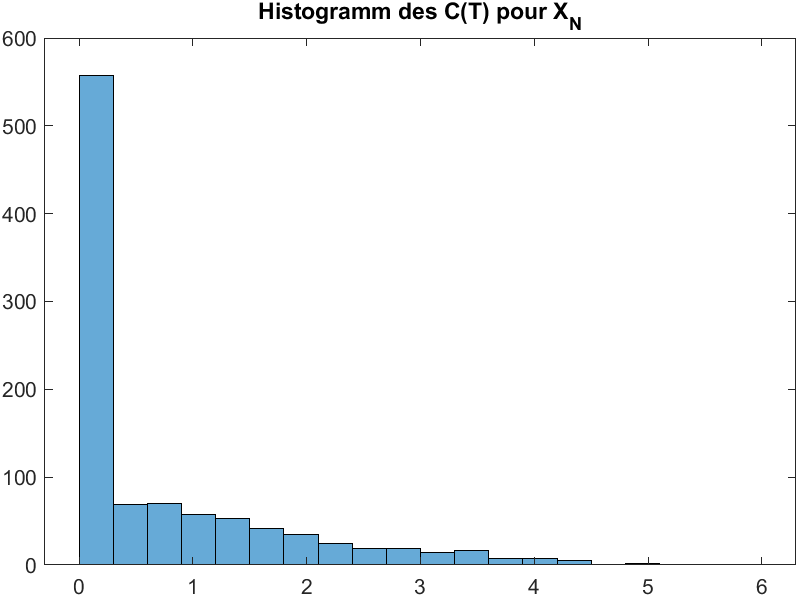
\includegraphics[width=14cm]{"graphiques/hist_C_N.png"}
    \caption{Histogramme des simulations pour $C_{N}$}
    \label{fig:hist_C_N}
  \end{center}
\end{figure}

\begin{figure}[h!]
  \begin{center}
    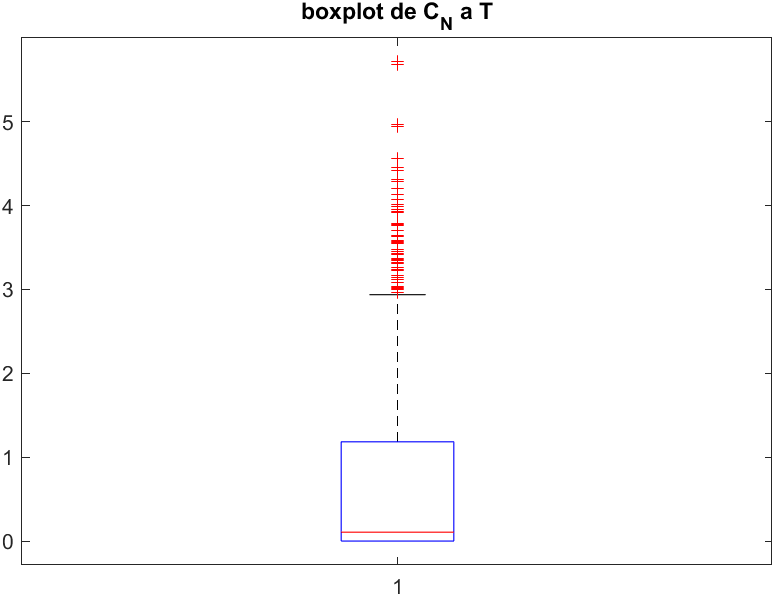
\includegraphics[width=14cm]{"graphiques/box_C_N.png"}
    \caption{Boxplot des simulations pour $C_{N}$}
    \label{fig:box_C_N}
  \end{center}
\end{figure}

\begin{figure}[h!]
  \begin{center}
    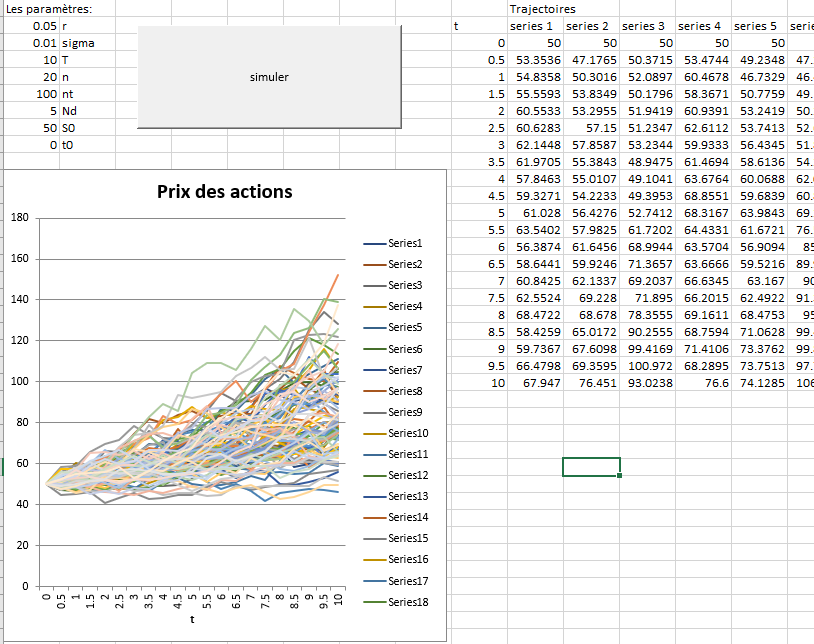
\includegraphics[width=14cm]{"graphiques/Capture.PNG"}
    \caption{le Excel dashboard}
    \label{fig:capture}
  \end{center}
\end{figure}


\section{Code Matlab}
\lstinputlisting{mini_projet.m}

\section{Code VBA}
\begin{lstlisting}[
    breaklines=true,
    tabsize=3,
    showstringspaces=false
    extendedchars=\true,
    language={[Visual]Basic},
    frame=single,
    framesep=3pt,%expand outward.
    framerule=0.4pt,%expand outward.
    xleftmargin=3.4pt,%make the frame fits in the text area. 
    xrightmargin=3.4pt,%make the frame fits in the text area.
    ]
Sub Macro1()

' parametres
Dim T, n, nt, Nd As Integer
Dim r, sigma, S0, t0 As Double

r = Range("A2").Value
sigma = Range("A3").Value
T = Range("A4").Value
n = Range("A5").Value
nt = Range("A6").Value
Nd = Range("A7").Value
S0 = Range("A8").Value
t0 = Range("A9").Value

Dim dt As Double
dt = ((T - t0) / n)

' premier cellule de la table de trajectoires ~ t0
Dim Srow, Scol As Integer
Dim Scol_abc As String
Srow = 3
Scol_abc = "I"
Scol = 9

' worksheets
Dim sh_dash, sh_calc, sh_s As String
Dim sh_dash_o As Worksheet
sh_s = "Dashboard"
sh_dash = "Dashboard"
Set sh_dash_o = Worksheets(sh_dash)

' iteratives
Dim i, j As Integer

Dim S() As Double
ReDim S(1 To n + 1, 1 To nt)
Dim dW As Double
Dim dS As Double
Dim x As Double

'effacer t et S() aines
With Worksheets(sh_s)
    Range(.Cells(Srow - 1, Scol), .Cells(Srow + 10000, Scol + 10000)).Delete
End With

' afficher t
Dim temps() As Double
ReDim temps(n + 2)
temps(0) = t0
For j = 1 To n + 2
    temps(j) = temps(j - 1) + dt
Next

Range(Scol_abc & Srow & ":" & Scol_abc & UBound(temps) + 1) = _
    WorksheetFunction.Transpose(temps)

'simuler et afficher S pas a pas
Cells(1 + 1, 9 + 0).Value = "t"
For j = 1 To nt
    x = S0
    i = 1
    Cells(2 + i, 9 + j).Value = x
    Cells(1 + i, 9 + j).Value = "series " & j
    For i = 1 To n + 1
        If i > 1 Then
            dW = Sqr(-2 * Log(Rnd())) * Cos(6.283185307 * Rnd()) * Sqr(dt)
            'dS = S(i - 1, j) * (r * dt + sigma * Sqr(S(i - 1, j)) * dW)
            'aine = Cells(1 + i, 10 + j).Value
            dS = x * (r * dt + sigma * Sqr(x) * dW)
            'S(i, j) = S(i - 1, j) + dS
            x = x + dS 'S(i - 1, j) + dS
            Cells(2 + i, 9 + j).Value = x
        End If
        S(i, j) = x
    Next
Next
'Range("J21:O100") = S()


' insert Chart
Worksheets(sh_s).Activate
Dim chartrange As Range
Set chartrange = Cells(Srow, Scol + 1)  'sans t
Set chartrange = chartrange.Resize(n + 1, nt)
MsgBox chartrange.Address

Worksheets(sh_dash).Activate
Dim Graphe As Object

'effacer graphes aines
For Each Graphe In ActiveSheet.ChartObjects
  Graphe.Delete
Next Graphe

Set Graphe = sh_dash_o.ChartObjects.Add( _
    Left:=Range("A11").Left, Width:=380, _
    Top:=Range("A11").Top, Height:=400)
With Graphe.Chart
    .SetSourceData chartrange
    .PlotBy = xlColumns 'echanger x et y axes
    .ChartType = xlLine
    .HasTitle = True
    .ChartTitle.Text = "Prix des actions"
    .FullSeriesCollection(1).XValues = _
        Range(Scol_abc & Srow & ":" & Scol_abc & UBound(temps) + 1)
    .Axes(xlCategory).HasTitle = True
    .Axes(xlCategory).AxisTitle.Text = "t"
End With


MsgBox "Simulation finie pour " & nt & " trajectoires."

'Sheets("Dashboard").Activate
'Range("Parametres").Select
'Range("A13").Value = T

End Sub

\end{lstlisting}



\end{document}
